\chapter{Implementation}
We implemented the Computer system in OMNeT++.\\
Our implementation consists of the following modules, also shown in \autoref{fig:omnetpp_implementation}:
\begin{itemize}
    \item \texttt{ProcessGenerator}: this module generates processes following the specified time distribution and sends them to the scheduler. The duration of each processing phase is also defined here.
    \item \texttt{scheduler}: this module handles the scheduling logic and keeps track of processes in their I-O phase.\\
    It contains an infinite-capacity queue. Depending on the \texttt{isFCFS} parameter, the queue is either a FIFO queue, when the parameter is set to true, or a priority queue whose elements are ordered by increasing duration.
    \item \texttt{cpu}: each of the $N$ CPUs, when it is free, receives a process from the scheduler and simulates its execution. When it finishes the execution phase (i.e. the I-O phase is reached or the process terminates), a message is sent to the scheduler, indicating that the CPU is now free.
\end{itemize}

\begin{figure}[H]
    \captionsetup{type=figure}
    \centering
    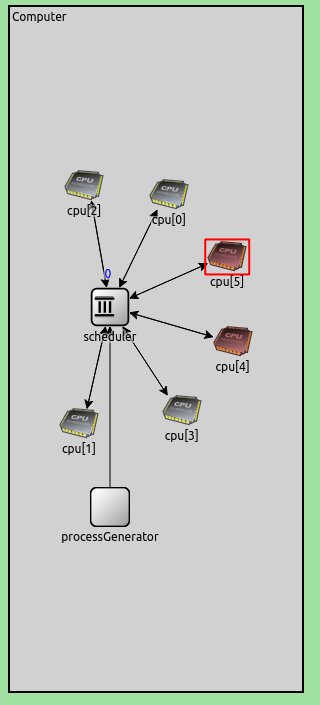
\includegraphics[width=0.4\textwidth]{images/example/sim_schema.png}
    \captionof{figure}{View of the system implementation in OMNeT++}
    \label{fig:omnetpp_implementation}
\end{figure}


